%!TEX root = ../template.tex
%%%%%%%%%%%%%%%%%%%%%%%%%%%%%%%%%%%%%%%%%%%%%%%%%%%%%%%%%%%%%%%%%%%%
%% chapter3.tex
%% NOVA thesis document file
%%
%% Chapter with a short latex tutorial and examples
%%%%%%%%%%%%%%%%%%%%%%%%%%%%%%%%%%%%%%%%%%%%%%%%%%%%%%%%%%%%%%%%%%%%

\typeout{NT FILE chapter3.tex}%


\chapter{Related Work}
\label{cha:related_work}


\section{3D WebGIS Apps for Digital Humanities}
\label{sec:webgis}

\subsection{The Turin 1911 Project}
\label{sec:turin_project} 


\subsection*{General Overview}

The "Turin 1911: The World's Fair in Italy" is a research project~\cite{spreafico20233d} led by the \textit{University of California San Diego} and  \textit{Politecnico di Torino} where a multidisciplinary team cooperates to document and investigate the 1911 World’s Fair held in Turin.
It integrates archival research, \gls{3D} reconstruction, and web\gls{GIS} technology to study and preserve the architectural and \gls{CH} of the Fair. Project URL: \url{https://arcg.is/1HfSqG} 

\subsection*{Process Description}

The web\gls{GIS} and \gls{GIS}-\gls{BIM} web apps are interactive tools to digitally navigate and query the environment. Below, there are the seps made to achieve both.
Three types of elements were used to create a \gls{3D} web\gls{GIS}: polygonal feature class, multi-patch feature class, or \gls{3D} object.

The historical map of the \textit{Valentino Park Fairground} was georeferenced and digitized, and a \gls{2D}/\gls{3D} map interface was developed using ArcGIS Online, allowing users to switch between views seamlessly. 
To develop the \gls{3D} models in \gls{BIM}-\gls{GIS} Web App, not only, photographs of each object, but also, plans, elevations, and sections of some Built Environment Objects, were collected. Using technical drawings, \gls{3D} models were generated and compared with historical photographs.
The final web\gls{GIS} application, for both dimensions, was created using ArcGIS Experience Builder configurable widgets(Figure \ref{fig:turin_study}).

\subsection*{Interactive Features}

Several tools were developed in the web\gls{GIS}, including a search bar, selection of \gls{2D} map/\gls{3D} scene, layer list, legend, navigation, filters, and pop-ups, allowing users to explore built environment objects. 
\gls{BIM} was used for detailed \gls{3D} reconstruction of selected Fair pavilions (e.g., Pavilion of Siam), and to create an interactive \gls{3D} scene with those layers. 
The actual shape of \textit{Valentino Park} was created from an aerial photogrammetric and processed in Agisoft Metashape. Applications like Experience Builder
enhanced interactivity, offering features like navigation and measurement tools, bookmarks, layer toggles, and camera orientation. The current geolocation enables users in the park to be located on the web\gls{GIS} and web app. 
The digitized archival materials are catalogued and linked to the geometries in a dedicated Geospatial Database. 
 

\begin{figure}[h!]
  \centering
  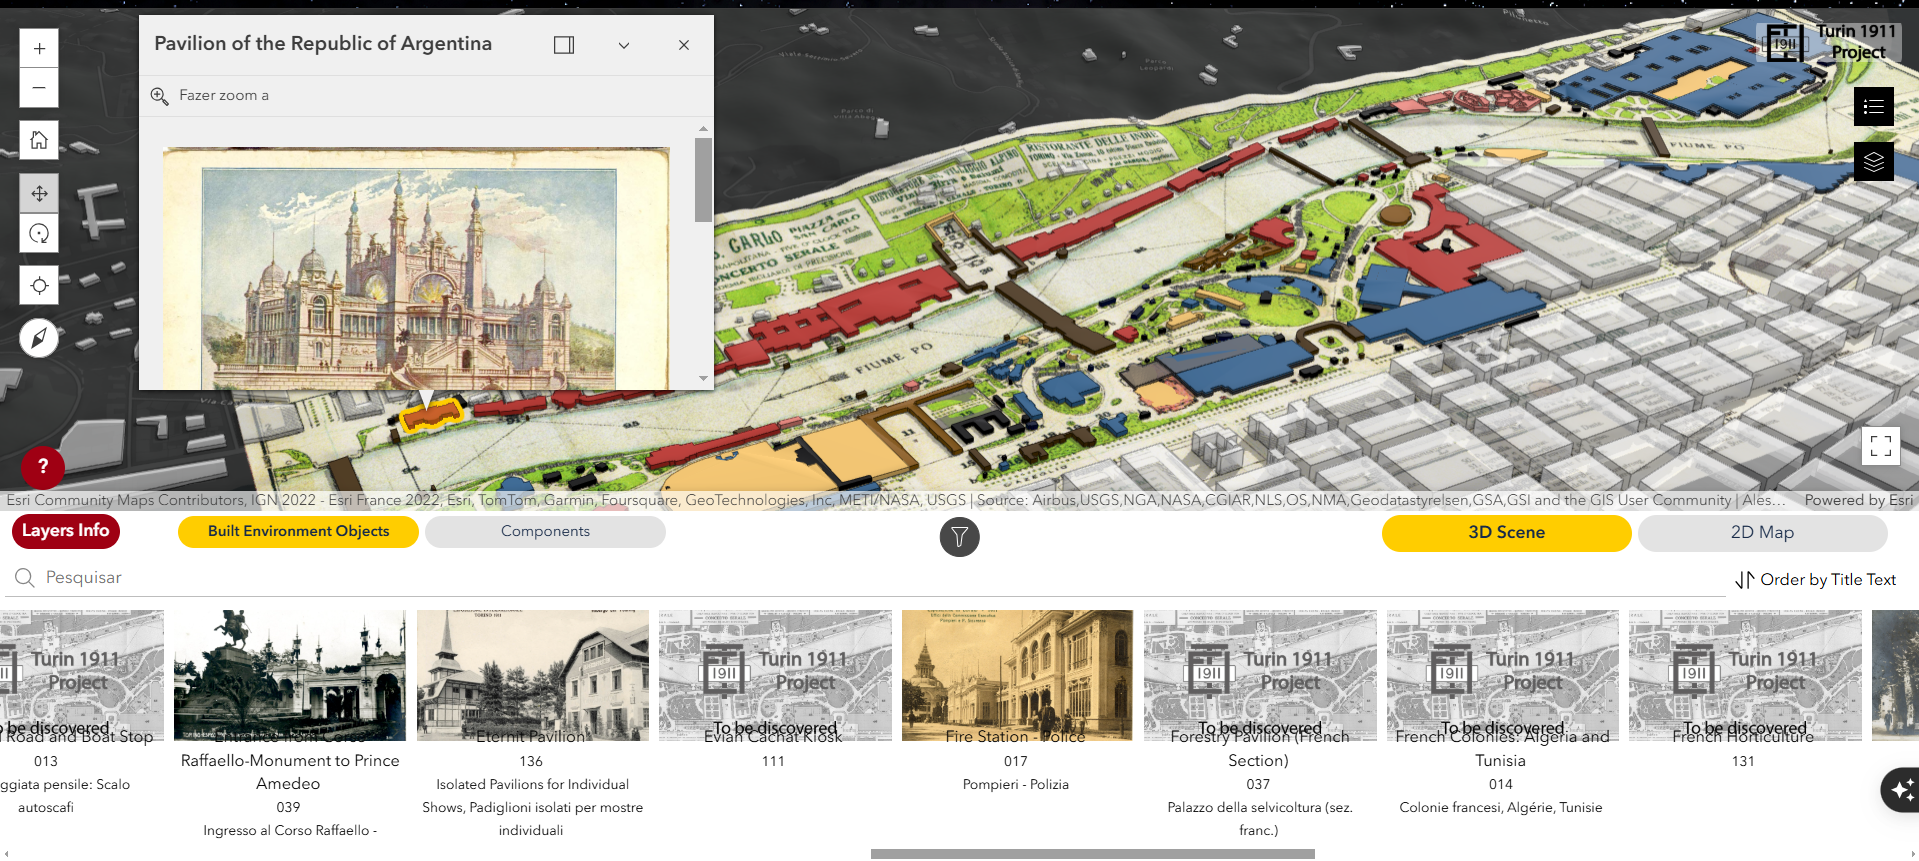
\includegraphics[width=0.8\linewidth]{turin_study}
  \caption{The \gls{2D}/\gls{3D} web \gls{GIS} Application}
  \label{fig:turin_study}
\end{figure}
\FloatBarrier



%\textbf{Limitations and Challenges}\\
%•	Data Conversion and Compatibilites:  Issues during transitions from the georeferencing model and coordinate system definition, and incompatibilities between products by ESRI itself.
%\\•	Software Compatibility: Frequent software updates, so compatibilities across the employed software must be verified before updating the entire system.
%\\•	Online vs. Enterprise GIS: ArcGIS Online presented limitations, such as the inability to directly link the webGIS to the geo-DB, which could be resolved in an Enterprise GIS setup.

\subsection{Web-Based \gls{GIS} for \gls{CH} of Safranbolu, Turkey} 
\label{sec:gis_safranbolu}

\subsection*{General Overview}

This study~\cite{arca2018development} focuses on the documentation and preservation of the \gls{CH} of Safranbolu, Turkey, a UNESCO World Heritage site\footnote{\url{https://whc.unesco.org/en/list/614/}}. 
The goal of this project is establish an internet-based information system and the \gls{GIS} modelling of all historical constructions of Safranbolu historical city.
This will be accomplished by compiling documentation and preservation of \gls{CH}, using \gls{GIS}, \gls{3D} models and digital photogrammetry.

\subsection*{Process Description}

The development stages of this work started with digital photogrammetry, where the objects coordinate system was defined, and control points marked on the ancient artifacts, and photographs of the antique artifacts taken.

Pictures then were transferred to computer and evaluated with photogrammetic software (\textit{Photomodeler}). Following this, the \gls{3D} modeling of the historical buildings was created.
\gls{3D} forms of the building were obtained using the photos form photogrammetry taken from different views, and the object models were covered with different surface and image textures.
\gls{GIS} was used to analyze spatial objects, such as buildings constructed within parcels and roads. The parcels were represented as polygons, while roads with lines.
The city map of Safranbolu was obtained in \gls{CAD} format, and then transferred to ArcGIS. This data was then evaluated in \gls{GIS} by building a topological infrastructure.
In the next phase of the project, all collected data—such as photos, videos, architectural drawings, and \gls{3D} and \gls{VRML} models—related to the selected historical buildings was prepared. 

This project integrates spatial data (e.g., building locations and \gls{3D} images) with non-spatial data (e.g., textual descriptions and historical information about the buildings) to document the historic town of Safranbolu. 
Through the interface (Figure \ref{fig:z}), users can visualize various types of data, including parcels, registered and non-registered buildings, roads, ownership details, addresses, and other relevant details about cultural monuments in the old Safranbolu area.

%\textbf{Technologies}\\
%•	Photomodeler 6.0 Used to create 2D and 3D models from taken photographs, using photos from several angles 
%\\•	ArcGIS server interfaces were used for design and develops of Web-server portal.


\begin{figure}
  \centering
  \begin{subfigure}[b]{0.45\textwidth}
      \centering
      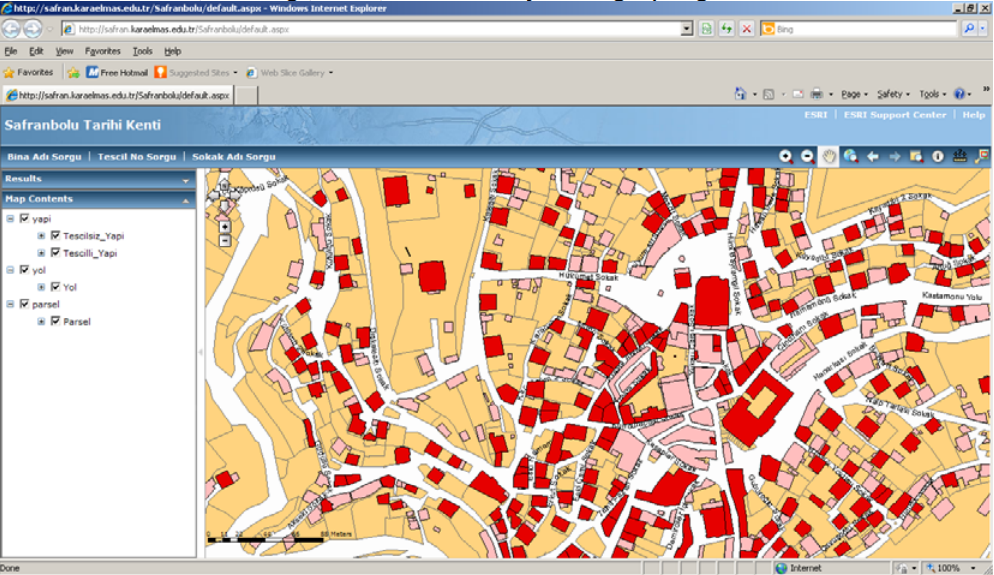
\includegraphics[width=1.0\textwidth, height=4cm]{turkey_thesis}
      \caption{Registered and non-registered buildings in the old Safranbolu area.}
      \label{fig:x}
  \end{subfigure}
  \hfill
  \begin{subfigure}[b]{0.45\textwidth}
      \centering
      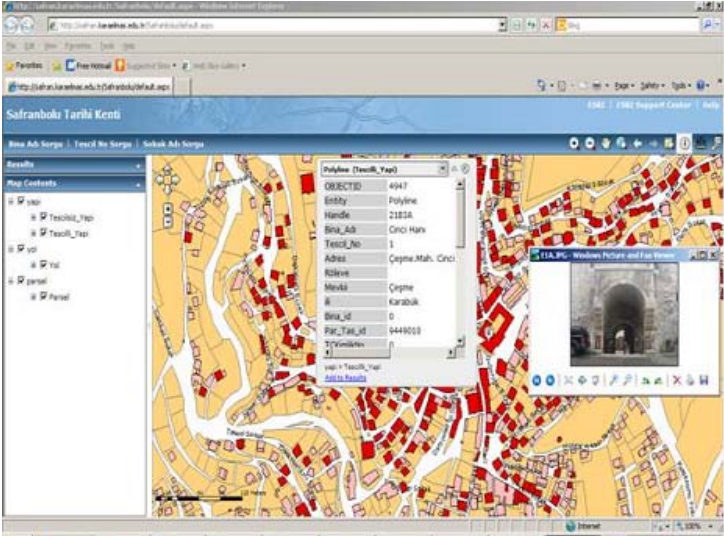
\includegraphics[width=1.0\textwidth, height=4cm]{test}
      \caption{Designed Web-based \gls{GIS} \textit{Cinci Caravanserai}.}
      \label{fig:y}
  \end{subfigure}
     \caption{Illustrative views of the Web-\gls{GIS} application.}
     \label{fig:z}
\end{figure}


% \begin{figure}[h!]
%   \centering
%   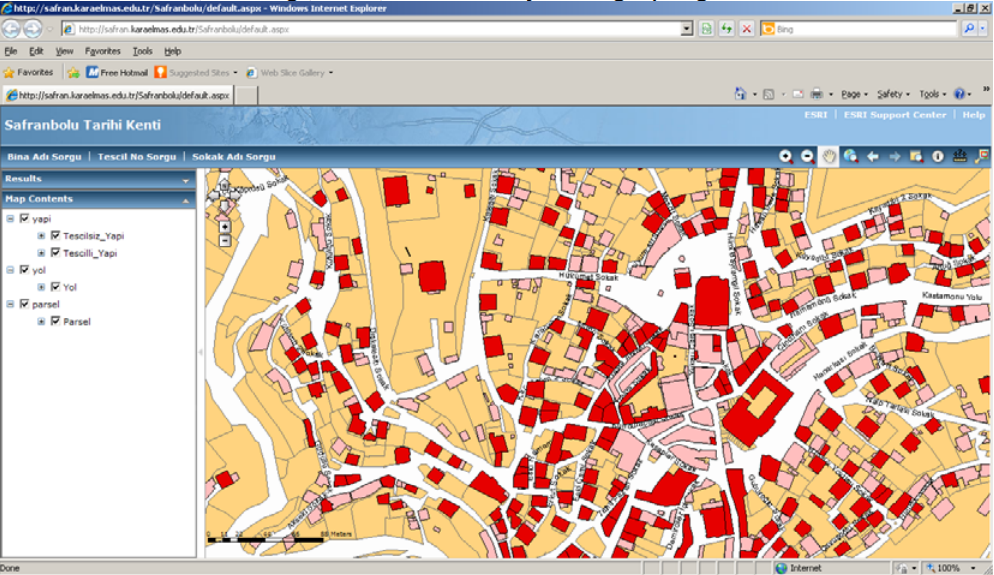
\includegraphics[width=0.8\linewidth]{turkey_thesis}
%   \caption{The view of registered and non-registered buildings in the center of old Safranbolu area.}
%   \label{fig:turkey_thesis}
% \end{figure}
% \FloatBarrier

% \begin{figure}[h!]
%   \centering
%   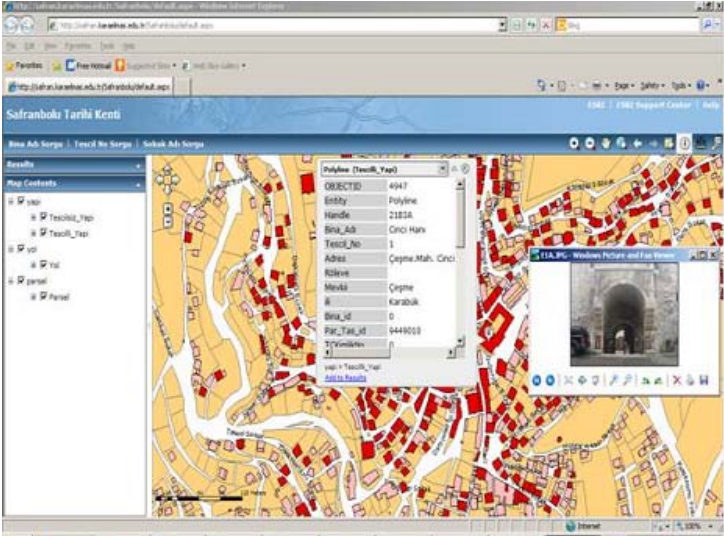
\includegraphics[width=0.7\linewidth]{test}
%   \caption{The view of registered and non-registered buildings in the center of old Safranbolu area.}
%   \label{fig:test}
% \end{figure}
% \FloatBarrier


\section{\gls{3D} in Cultural Heritage and Virtual Reality}
\label{sec:3d_vr}

\subsection{\gls{VR} Scenario with Funerary Artifacts from Ancient Egypt} 
\label{sec:3d_vr_devices}

\subsection*{General Overview}

This research~\cite{gonizzi20153d} leverages \gls{VR} to enhance the accessibility and understanding of Egyptian funerary artifacts in the Sforza Castle, Milan. 
Aimed at exhibition renewal, the project creates an immersive \gls{VR} experience to engage visitors of the “Archaeological Museum” in Milan, with the ancient Egyptian "Path of the Dead" ritual, integrating interactive \gls{3D} models and hieroglyphic translation tools. Four key funerary artifacts were used for their historical and archaeological significance:
\begin{itemize}
  \item \textbf{Ushabty}: statuettes (pharaoh, minister)
  \item \textbf{Heart Scarab}: amulet
  \item \textbf{Wooden sarcophagus} 
\end{itemize}


%\textbf{Context} \\
%The project is still ongoing, and the results presented in this paper are the first step to a complete implementation and real installation in the Museum. 

\subsection*{Process Description}

Firstly, the photogrammetry was built by moving the camera all around these objects to capture all angles. Subsequently, the software \textit{Agisoft Photoscan} was used for texture blending. Then, the output file was imported into \textit{Adobe Photoshop} for word delineation, outlining and identification. 
Finally, \textit{Polyworks} to simplify the model, and resolution/texture optimization.
The \gls{VR} device Oculus Rift DK2 provided stereoscopic visualization, while Leap Motion tracked hand movements for object interaction (grabbing, rotating, and highlighting).

The responsive \gls{POI} were exported in \textit{fbx} format, and the cut parts were then imported to Unity, for integration as \gls{3D} models.
The \gls{POI} highlight cultural symbols and texts on artifacts (e.g., religious inscriptions). When selected, they provide detailed descriptions and explanations.
The computer graphics program \textit{\gls{3D} Studio Max} was used to enhance specific elements of the models, to improve hieroglyphs readability.
Touch-Triggered Transliteration and Translation allows users to interact with hieroglyphic symbols. If the user wants to know more about these words, it can touch the part, the word is automatically enhanced and the transliteration and the following translation appears as illustrated in Figure \ref{fig:vrGis_thesis2}. The data involved is the name of the deceased, and descriptions explaining images or drawings on the objects.
Users can rotate and grab the \gls{3D} models using hand gestures, as shown in Figure \ref{fig:vrGis_thesis1}.


\begin{figure}
  \centering
  \begin{subfigure}[b]{0.45\textwidth}
      \centering
      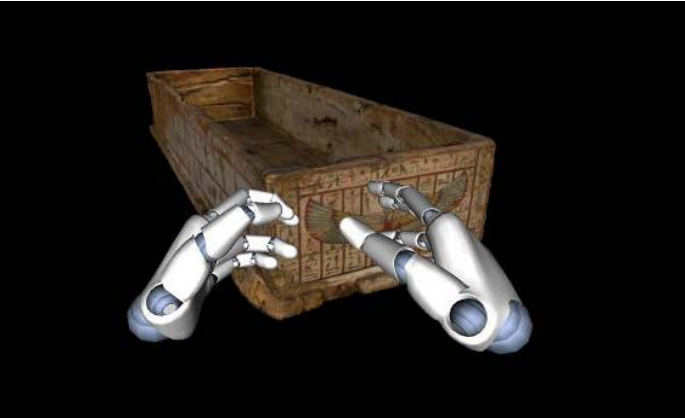
\includegraphics[width=1.0\textwidth, height=4cm]{vrGis_thesis1}
      \caption{Grabbing and rotating the object.}
      \label{fig:vrGis_thesis1}
  \end{subfigure}
  \hfill
  \begin{subfigure}[b]{0.45\textwidth}
      \centering
      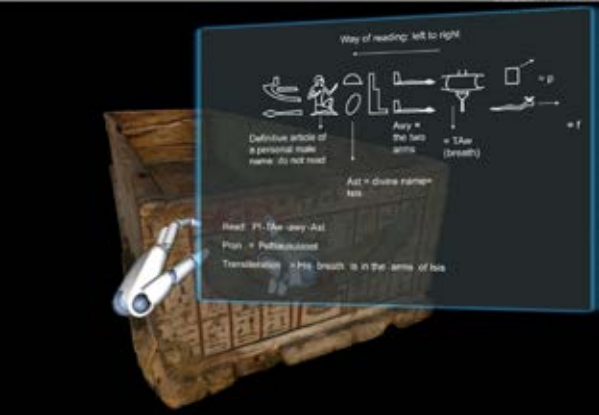
\includegraphics[width=1.0\textwidth, height=4cm]{vrGis_thesis2}
      \caption{Highlighting and translation the text.}
      \label{fig:vrGis_thesis2}
  \end{subfigure}
     \caption{Visual representations of the implemented \gls{VR} scenario}
     \label{fig:vrGis_thesis}
\end{figure}


%\textbf{Project Objectives} \\
%•	Better understanding of Egypt funerary objects by proposing an interactive translation of the language of ancient Egyptians(hieroglyphics)
%\\•	Deliver an engaging and educational museum experience through VR.

% \textbf{User Feedback} \\
% Preliminary tests done by involving students and researchers.
% Conclusions: \\
% •	Some of the test users have tried a slight feeling of nausea after a prolonged use of the system Oculus + Leap Motion, due to the high latency and the low resolution of the display.
% \\•	During the first tests, the words were difficult to be read since they were blurry and therefore not understandable. The problem was solved using widgets as a pop-up window.

%\textbf{6. Comparison and Limitations} \\
%Key Limitations: \\
%•	Hardware constraints (e.g., resolution and latency of Oculus Rift DK2).
%\\•	Limited depth of hieroglyphic translations in the current stage.

% \textbf{Future Work} \\
% Planned Developments: \\
% o	The future works involve the creation of an immersive "Path of the Dead" virtual environment where the models of the objects already processed will be inserted, integrated with other models. The level of information provided will be increased with other translation and description, to provide a better and deepened comprehension of the information.



\section{Related Theses}
\label{sec:thesis_nova}


At NOVA, recent theses have consistently focused on integrating digital tools into museums, aiming to offer immersive experiences through \gls{VR} technology or \gls{3D} media visualizations 
of \gls{CH} objects, often incorporating interactive maps, an approach that will be implemented in my dissertation. Over the past year, two theses have explored how to 
present a virtual tour of museums. The third one, developed by Joao Vilar, explored interactive games, with an emphasis on cultural artifacts from the Portuguese Évora site.


\subsection{\textit{Sistema para Criação e Exploração de Narrativas Interativas e Jogos} – João Vilar}
\label{sec:thesis1_nova}


In 2022, João Vilar developed a thesis as part of \gls{PASEV} \footnote{\url{https://pasev.hcommons.org/}}. \gls{PASEV} is a project that analyses new perspectives regarding the cultural manifestations of the UNESCO patrimonial city of Évora,
which has a significant historical context. The project started by Rosário and extended by Ferreira started with the development of a historical soundscape's web platform \footnote{\url{https://pasev.uevora.pt/}}. 
This work focused on the study of sound events that occurred from 1540 to 1910 with the aim to preserve the city's auditory heritage and its significant historical context. The user can
visualize and display audio and media in the web platform. ~\cite{rodrigues2021using}

  
This thesis expanded the existing \gls{PASEV} platform by introducing JoNI, an infrastructure designed to support the creation of an interactive game. In the end of this project, a mobile 
application was developed incorporating games with a narrative and characters, including \gls{2D}/\gls{3D} models and auditory data, and object recognition via photos. There were developed two 
functional prototypes. The first, an interactive card game that teaches music instruments through audio and visual elements. The second, a gamification app to promote the discovery 
of diverse locals with their itineraries.  Along the route, textual content, videos, audios and a ranking progress are reproduced to make an interactive and learnable experience. 
For each game, two main tabs were implemented for managing the map and \gls{AR} features of the game. ~\cite{tese_jogosVilar2022}

This implementation includes \gls{AR} and geolocation technologies to immerse users in Évora's \gls{CH}.~\cite{vilar2024extended}
The solution was built on top of an existing base map. Afterward, the \gls{POI} of Évora were identified and represented with \gls{AR} markers. Additionally, GPS tracking was
  integrated to allow users to monitor their location.
The solution integrates a native Android environment and Unity game engine for seamless communication. The main goal of this dissertation is the dissemination of the \gls{CH} 
and soundscape of Évora, with the solution integrated into Museu Nacional Frei Manuel do Cenáculo (MNFMC) \footnote{\url{https://www.museusemonumentos.pt/pt/museus-e-monumentos/museu-nacional-frei-manuel-do-cenaculo-e-igreja-de-nossa-senhora-das-merces}}. 
The database was extended using PostgreSQL and PostGIS technologies.
This project intersects with my dissertation, which explores the digital representations of cultural artifacts, and the dissemination of historical studies related to a Portuguese site. 
Both involve the creation of a digital map and \gls{3D} object representations with tactile/auditory interactions.

\subsection{Designing and implementing a museum Virtual Tour, Museu dos Coches – José Coimbra}
\label{sec:thesis2_nova}

This thesis involved the development of a \gls{VE} that simulates a museum visit, providing an immersive and interactive user experience. The project integrates a \gls{3D} environment 
with \gls{3D} scanned objects, complemented by an intuitive and user-friendly interface. 
This virtual tour was based on the National Coach Museum\footnote{\url{http://museudoscoches.gov.pt/pt/}} and performs as a model for \gls{VR} museum environments. This approach can revolutionize 
museum tours, suggesting an alternative, immersive, and innovative platform for cultural enrichment. 
The technologies used include Unity to create and deploy the \gls{VE}, and the virtual visit requires a \gls{VR} headset equipped with hand-tracking capabilities. For this purpose, 
the Meta Quest 3 Headset \footnote{\url{https://www.meta.com/quest/quest-3/}} was used to improve the processing power over earlier models. Therefore, this software ensures an optimized \gls{VR} experience. ~\cite{tese_tourCoimbra2024}
This thesis has some points in common with this one and was elaborated in 2024. Both use digital tools for an interactive user experience with \gls{CH} elements.


\subsection{Web integration of virtual museums tours and \gls{3D} media visualization, Academia das Ciências – Nelson Faria}
\label{sec:thesis3_nova}

Last year, the following thesis was developed in collaboration with the Academia das Ciências de Lisboa\footnote{\url{https://www.acad-ciencias.pt/}} one of the oldest scientific institutions in Portugal, active since 1779.~\cite{tecnicoAcademia} 
The academy is dedicated for promoting and preserving \gls{CH}, with both physical and digital collections accessible to the public. 
The project focuses on integrating \gls{CH} objects in \glspl{VE}. As part of this work, a website was created to provide a virtual tour of the academy, presenting its spaces and \gls{CH} objects in an engaging and informative manner.~\cite{tese_tourFaria2024} 
This website is available at the following URL: \url{https://visita3d.acad-ciencias.pt/} 
Designed with a user-friendly interface, the website offers an intuitive navigation experience, including an audio guide with simulated narration, background music, a \gls{3D} viewer, and the user can explore the components and history behind each artifact. 
~\cite{academiaCiencias2024} The project also incorporates an interactive itinerary map, displaying all the available rooms and buttons for instinctive control of the tour. This feature allows users to explore the academy's diverse spaces quickly and effectively.
Matterport technology was employed to create the visualization and interaction environments, providing \gls{3D} spatial mapping of the academy's rooms. Complementing this, \gls{3D} object models were created and displayed in a Sketchfab viewer. 
To support these features, several technologies were used, including Matterport Pro3 Camera for the \gls{3D} scanning and 360º immersive views, along with frontend and backend frameworks, including Vue.js and Tailwind CSS for the interface, 
while the backend relied on Node.js. In addition, it was implemented a database to store and manage the media content.

\subsection{Developing support for digital representations of Heritage artefacts in cultural exhibitions – Márcia Campanha}
\label{sec:marcia_thesis}

This thesis~\cite{campanha2024heritage} pretended to extend the work of Tiago Nunes, by enhancing user interaction with 
artifacts in the \gls{VE}. The functionalities focus on object interaction, such as the ability to apply different textures, the possibility to manipulate specific parts of the object independently, and access detailed information regarding each one.
Users can manipulate objects through the three axes(X,Y,Z) by rotating, scaling, or translating them within the virtual space.
To obtain detailed information of the antiquities, the user simply selects the desired component.
Additionally, users can upload the pretended object to the virtual exhibition and view a gallery menu displaying multiple perspectives of the \gls{3D} models of the same artifact.
The system allows users to apply different textures to individual object components and select specific parts, which are outlined with their associated descriptions.
The full interface, including these interactive features, can be observed in Figure \ref{fig:marcia_image}.
This project will be integrated into my thesis to support the \gls{3D} manipulation of object models and facilitate the archaeological analysis of the various components of each glass artifact.

\begin{figure}[h!]
  \centering
  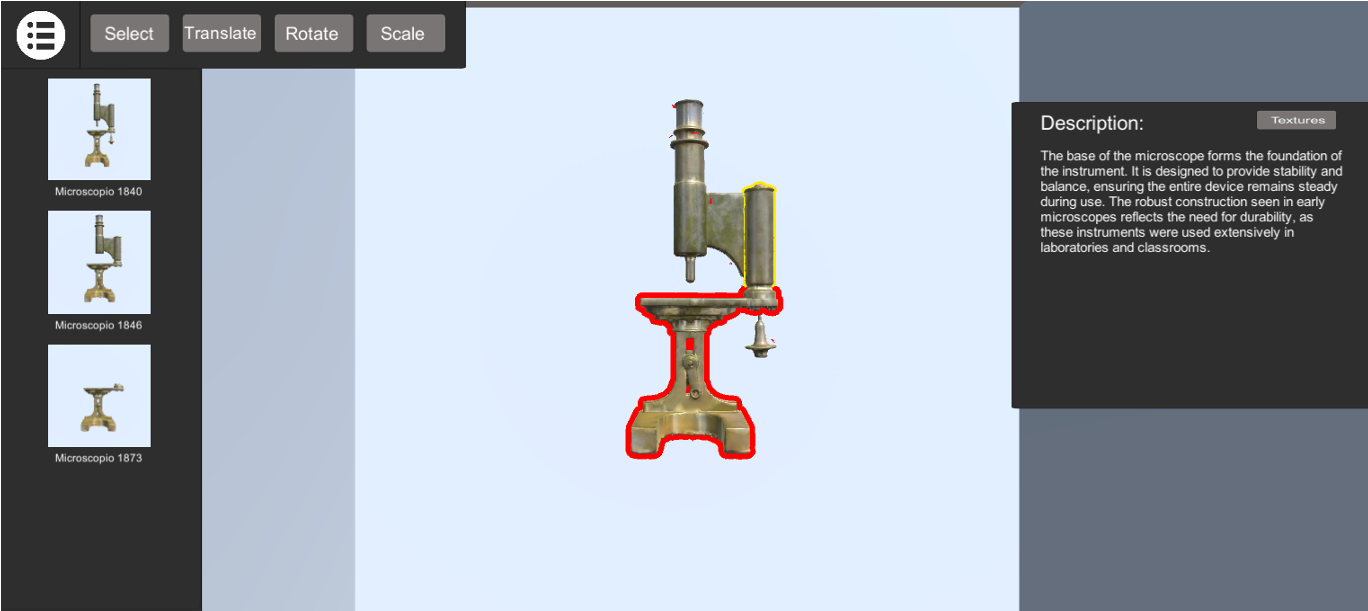
\includegraphics[width=0.8\linewidth]{marcia_thesis}
  \caption{Interface for interacting with heritage artifacts.}
  \label{fig:marcia_image}
\end{figure}
\FloatBarrier


\section{Discussion}
\label{sec:discussion}

\newcommand{\cmark}{\ding{51}} % Checkmark
\newcommand{\xmark}{\ding{55}} % Cross

\begin{table}
  \resizebox{\textwidth}{!}{
  \small
  \centering
  \begin{tblr}{
    colspec={lccccc},
    hlines
  }
  \textbf{Project Name}                            & {\textbf{Interactive} \\ \textbf{Map}} & {\textbf{3D Models} \\ \textbf{Interaction}} & {\textbf{AR/VR} \\ \textbf{Experience}} & {\textbf{Data} \\ \textbf{Repository}} & {\textbf{Virtual} \\ \textbf{Tour}} \\
  \hline
  Turin 1911 Project                               & \cmark  & \cmark  & \xmark  & \xmark  & \xmark  \\
  Safranbolu GIS                                   & \cmark  & \xmark  & \xmark  & \xmark  & \xmark  \\
  VR Funerary Artifacts                            & \xmark  & \cmark  & \cmark  & \xmark  & \xmark  \\
  JoNI (PASEV)                                     & \cmark  & \cmark  & \cmark  & \cmark  & \cmark  \\
  Museu dos Coches Virtual Tour                    & \xmark  & \cmark  & \xmark  & \xmark  & \cmark  \\
  Academia das Ciências 3D View                    & \xmark  & \cmark  & \xmark  & \xmark  & \cmark  \\
  Digital Representations of Heritage Artifacts    & \xmark  & \cmark  & \cmark  & \xmark  & \xmark  \\  
  \end{tblr}
  }
  \caption{Comparison of Projects Functionalities}
  \label{tab:comparison2}
\end{table}


% \begin{table}[h]
%   \centering
%   \scriptsize
%   \begin{tabular}{lcccccc}
%   \toprule
%   \textbf{Project Name} & \textbf{Interactive Map} & \textbf{3D Models} & \textbf{AR/VR Experience} & \textbf{GIS Integration} & \textbf{Data Repository} & \textbf{Virtual Tour} \\
%   \midrule
%   Turin 1911 Project & \cmark & \cmark & \xmark & \cmark & \xmark & \xmark \\
%   Safranbolu GIS (Turkey) & \cmark & \xmark & \xmark & \cmark & \xmark & \xmark \\
%   VR Funerary Artifacts (Ancient Egypt) & \xmark & \cmark & \cmark & \xmark & \xmark & \xmark \\
%   Criação de Narrativas Interativas e Jogos (PASEV) & \cmark & \cmark & \cmark & \xmark & \cmark & \cmark \\
%   Museu dos Coches Virtual Tour & \xmark & \cmark & \xmark & \xmark & \xmark & \cmark \\
%   Academia das Ciências 3D Visualization & \xmark & \cmark & \xmark & \xmark & \xmark & \cmark \\
%   \bottomrule
%   \end{tabular}
%   \caption{Comparison of Functionalities}
%   \label{tab:comparison}
%   \end{table}

